%File: formatting-instruction.tex
\documentclass[letterpaper]{article}
\usepackage{aaai}
\usepackage{times}
\usepackage{helvet}
\usepackage{courier}
\usepackage{amsmath}
\usepackage{amssymb}
\usepackage{amsfonts}
\usepackage{algorithm}
\usepackage{algorithmicx}
\usepackage{algpseudocode}
\usepackage{amsthm}
\usepackage{natbib}
\usepackage{textcomp}
\usepackage{graphicx}

\theoremstyle{plain} \newtheorem{theorem}{Theorem} \newtheorem{proposition}{Proposition} \newtheorem{lemma}{Lemma}
\newtheorem*{corollary}{Corollary}  \newtheorem{claim}{Claim} 

\theoremstyle{definition} \newtheorem{definition}{Definition} \newtheorem{conjecture}{Conjecture} \newtheorem*{example}{Example} 

\theoremstyle{remark} \newtheorem*{remark}{Remark} \newtheorem*{note}{Note} \newtheorem{case}{Case}

\newcommand{\R}{\mathbb{R}}

\frenchspacing
\pdfinfo{
/Title (Faster Optimal Planning with Partial-Order Pruning)
/Subject (AAAI Publications)
/Author (Redacted)}
\setcounter{secnumdepth}{0}  
 \begin{document}
% The file aaai.sty is the style file for AAAI Press 
% proceedings, working notes, and technical reports.
%
\title{Faster Optimal Planning with Partial-Order Pruning}
%%\author{AAAI Press\\
%Association for the Advancement of Artificial Intelligence\\
%2275 East Bayshore Road, Suite 160\\
%Palo Alto, California 94303\\
%}
\author{}

\maketitle
\begin{abstract}
\begin{quote}
  When planning problems have many kinds of resources or high
  concurrency, each optimal state has exponentially many minor
  variants, some of which are "better" than others. Standard methods
  like A* cannot effectively exploit these minor relative differences,
  and therefore must explore many redundant, clearly suboptimal
  plans. We describe a new optimal search algorithm for planning
  that leverages a partial order relation between states. Under
  suitable conditions, states that are dominated by another with
  respect to this order can be pruned while provably maintaining
  optimality. We also describe a simple method for automatically
  discovering compatible partial orders in both serial and concurrent
  domains. In our experiments we find that more than 99\% of search
  states can be pruned in some domains.
\end{quote}
\end{abstract}

\section{Introduction}

Planning problems differ from other search problems in a number of
ways. One important distinction is that there are typically many
planning states that are ``similar'' along one or more dimensions.
For instance, in a job shop scheduling domain, one search state
might have the same number of widgets---but fewer sprockets---than
another. Assuming that more is always better and that the two states
can be reached in the same time, we can safely discard the former,
\textit{dominated} states, instead focusing our search on the better
state.

In this paper, we seek to formalize this notion, using Pareto
dominance to prune states that are strictly dominated by some other
states. More specifically, we give conditions under which we can
expand only those states in the \textit{skyline}, that is, states
that are not dominated by any another state. Our system, Skyplan,
is a refinement of Uniform Cost Search or A$^*$ that expands only
those states that are on the skyline.

The central idea underlying our approach is to define a partial
order relationship between states in the search space. This partial
order has an intuitive interpretation: one state dominates another
if it has no fewer ``good'' resources (e.g. jobshop outputs) than
another, no more ``bad'' resources (e.g. labor expended or time
taken), and it is better in one or more ways. 

In addition to proving the correctness of our approach, we also
show how to automatically infer such a partial order from a problem
specification such as PDDL.~\cite{ghallab1998pddl,fox2003pddl2}
This procedure is fairly intuitive: one simply needs to determine
which resources or propositions are uniformly good or bad, and---for 
domains with durative actions---which actions have uniformly
good or bad final effects.

In our experiments, we compare Skyplan to a similar implementation
of $A^*$ on several (XXX) job shop domains. In addition, we introduce
two new domains, based on the popular video game StarCraft. (XXX
we should credit evo chamber for one of them.) Skyplan performs
especially well in these scenarios, cutting the branching factor
by as much as 99\% compared to A$^*$.  Furthermore, we compare our
algorithm to a heuristic open source planner specifically engineered
to one of the two StarCraft domains.

\section{Skyplan}

\begin{figure}
	\begin{center}
	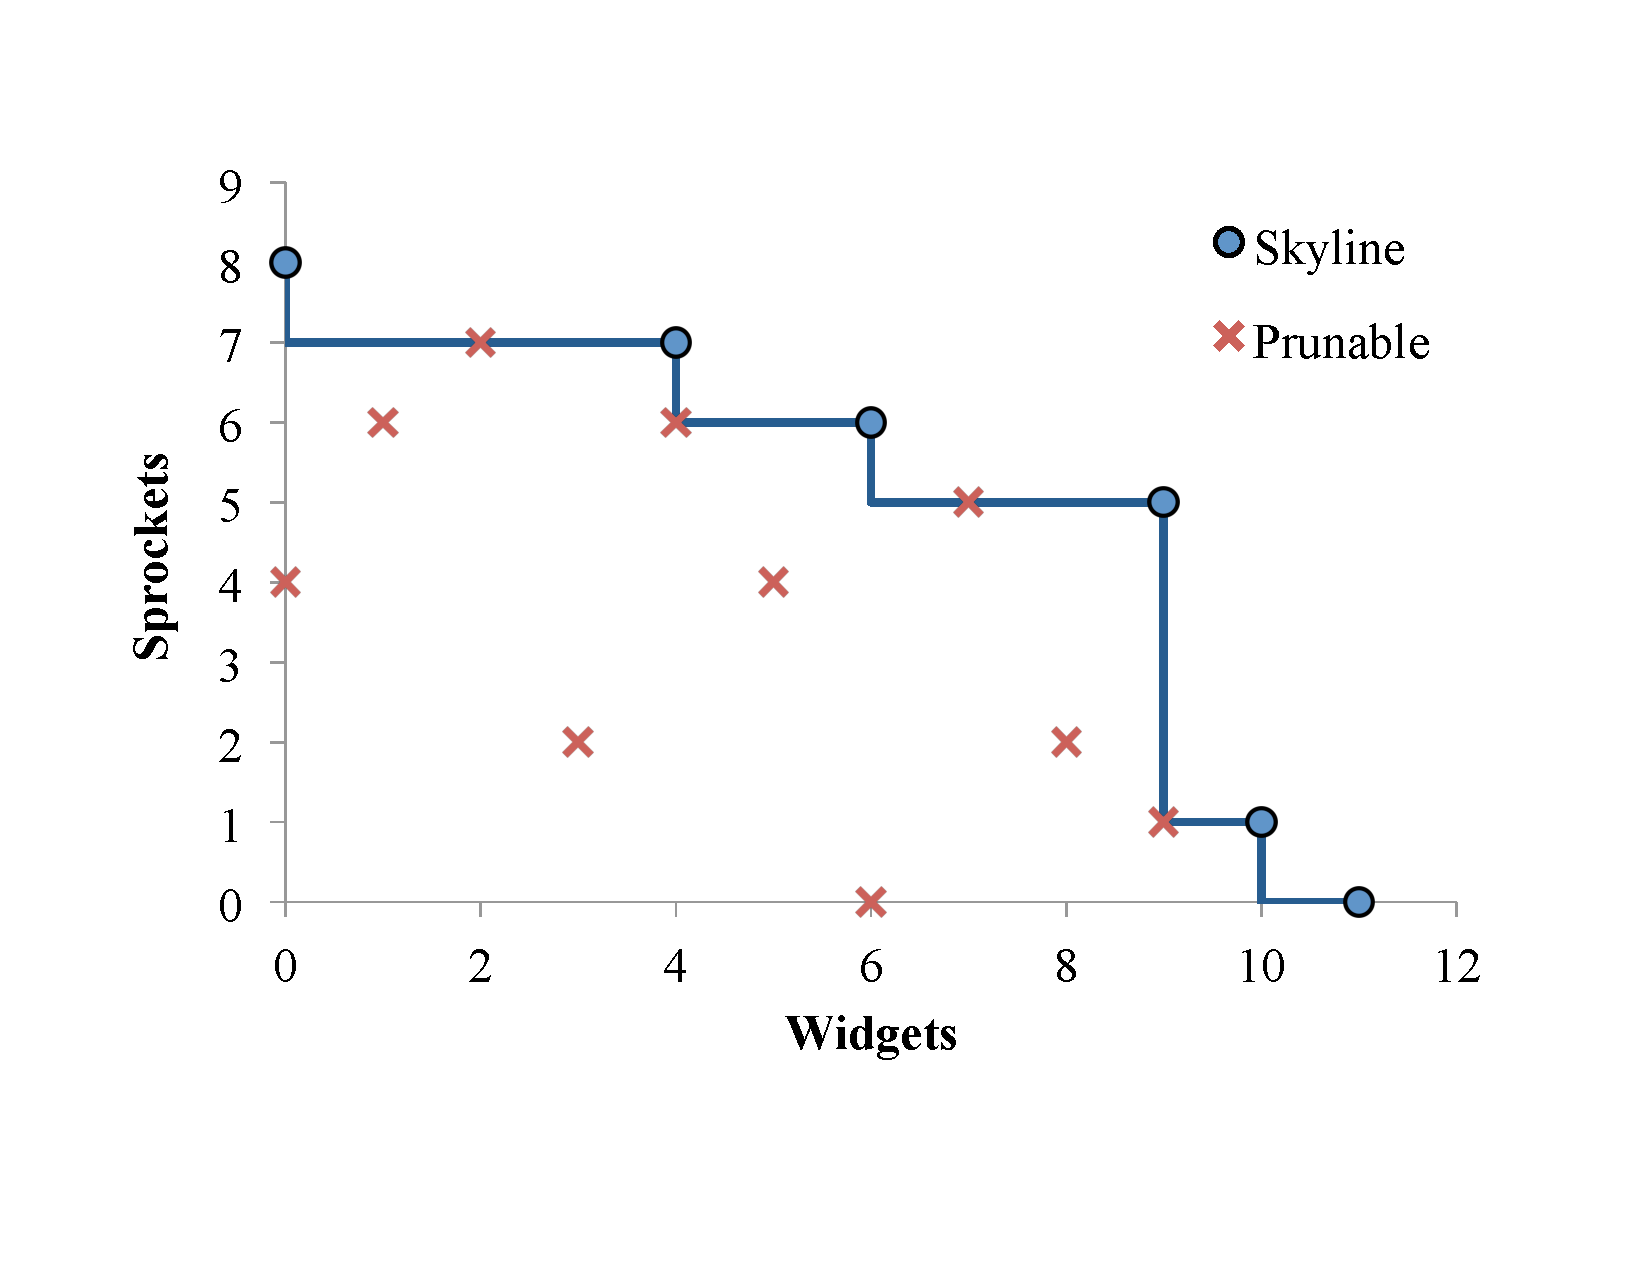
\includegraphics[width=3.3in]{skyline2d.pdf}
\end{center}
  \caption{An example set of states in a two-resource planning domain. If
all pictured states have the same cost, then only those shown as circles are
worth exploring; the xes can be safely pruned.}
\end{figure}

We operate in the standard convention of planning as search within
a weighted directed graph.  A planning problem consists of a directed
graph $G$ with states $n$ consisting of planning states.  States are
linked by directed edges with an associated a cost function
$\mathrm{cost}(n_s,n_t) \in \mathbb R^+$.  There is also a privileged
initial state $s$, along with a set of goal states $F$.  Further
define $g(n)$ to be the minimum cost path from $s$ to any state $n$.
Our goal is to find a path from $s$ to some state $n_g \in F$ with
the lowest g cost.


\subsection{Partial Orders}

We will further assume that our graph is endowed with a partial order $\preceq$
that relates states $n$ to one another, with the intuitive semantics that
$n \preceq m$ if $n$ is no better than $m$ in any way. For example, in
our sprockets and widgets example, $n \prec m$ if $n$ has no more widgets and
no more sprockets than $m$ and if $g(n) \ge g(m)$. Strict dominance
holds if $m$ is in addition strictly better than $n$ in some way.

Our goal is to define an optimal search algorithm that can exploit
this partial order to reduce the search space by only expanding
states $n$ that are \textit{weakly Pareto optimal}, that is states
$n$ with $n \nprec n^\prime$ for all states $n^\prime$. For any set of states
$N$, we define the \textit{skyline} of that set as
$\textrm{skyline}(N)=\{n: \ne n^\prime \in N: n \prec n^\prime\}$. That is, the
skyline of a set is those states which are weakly Pareto optimal.
In subsequent sections, we will give a useful sufficient condition
under which we can exploit a partial order while preserving correctness
of optimal graph search algorithms.

We are not the first to suggest the use of Pareto optimality or
skyline queries in the context of planning. For example, the
non-optimal Metric-FF planner~\cite{hoffmann2003metric} employed a
more limited notion of dominance, requiring that all propositions
be the same between two states, the domain to be monotonically
``good'' in all resources, and for the dominating state to have no
fewer resources along any axis. Our notion of dominance is more
general, and we are able to find useful partial orders in more general
domains.

More recently, in another satsificing planner, \citet{roger2010more}
combined multiple heuristics by only expanding those states which
were currently Pareto optimal with respect to the current open set.
By contrast, we seek to \textit{prune} search states while still
maintaining optimality.

Still others have employed other notions of partial orders while
maintaining completeness and optimality. These methods largely fall
into a category known as ``partial order reduction techniques,''
from computer aided verification. These methods fall into two
categories: those that prune states and those that prune transitions.
The former class includes expansion cores \cite{chen09completeness,
xu11theory}, which select only ``relevant'' actions for any given
state. The latter consists of methods like commutativity
pruning~\cite{geffner2000admissible}, which prunes redundant
permutations of partial plans, and stratified
planning~\cite{chen2009stratified}, which identifies layers of the
planning problem and only considers actions appropriate to a given
layer. \citet{wehrle2012partial} recently showed that all of these
techniques are special cases of more general techniques from computer
aided verification, namely sleep sets~\cite{godefroid96partial} and
stubborn sets~\cite{valmari92stubborn}. These methods are largely
orthogonal to our approach. Indeed we use something not unlike
expansion cores in our system.


\subsection{Algorithm}

Skyplan is a fairly straightforward modifications of Uniform
Cost Search or A$^*$. For the sake of exposition, we focus on Uniform Cost
Search, though A$^*$ or any optimal graph search algorithm can
be modified in the same way.

Skyplan is defined in Algorithm \ref{alg:skyplan}. Essentially, we run Uniform Cost Search as normal, except that 
we only expand states that are not strictly dominated by another
state we've either expanded or enqueued for expansion. That is, we only expand nodes that are in the \textit{skyline}
of the nodes explored so far.

\begin{algorithm}
  \begin{algorithmic}[1]
    \Procedure{Skyplan}{XXX}
    \State Initialize $Open=\{\langle s,0\rangle\}$, $Closed=\{\}$, $Pruned=\{\}$
    \While{ $Open$ is not empty}
    \State Pop the minimum cost state $\mathbf{n} = \langle n,c\rangle\in Open$
      \State $n\rightarrow Closed$
      \If {$n\in F$} 
        \State \Return the path to $n$ following back pointers
      \EndIf
      \For {$n^\prime\in\mathrm{succ}(n)$} 
      \State $\mathbf{n^\prime} \gets \langle n^\prime,c+\mathrm{cost}(n,n^\prime)\rangle$
        \If {$\forall m \in Open \cup Closed. n^\prime \nprec m$}
        \State $\mathbf{n^\prime} \rightarrow Open$
        \EndIf
      \EndFor
    \EndWhile
  \EndProcedure
  \end{algorithmic}
\caption{Skyplan}
\label{alg:skyplan}
\end{algorithm}

\subsection{Compatibility}
\begin{figure}
  \caption{Compatible partial orders. Partial orders stay ahead.}
\end{figure}

Not just any partial order on states can be used to preserve optimality. As a perverse
example, we can define a partial order under which all states on the optimal path
are dominated by non-optimal states. Thus, we need to define a property
under which a partial order is \textit{compatible} with a search graph. While
a broad class of partial orders might work, we have identified a particular 
property that is especially applicable to planning problems:

\begin{definition}[Compatibility]
	\label{def-compatibility}
  A partial order $\prec$ is \textit{compatible} if for all states $n \preceq m$,
  \begin{enumerate}
    \item $g(n) \ge g(m)$, and 
    \item $\forall n^\prime \in \mathrm{succ(n)}$ $\exists m^\prime \in
      \mathrm{succ}(m^\prime)$ such that $n^\prime \preceq m^\prime$ and
      $cost(n,n^\prime) \ge cost(m, m^\prime)$, and
    \item If $n \in F$, then $m \in F$
  \end{enumerate}
\end{definition}
This recursive definition of compatibility essentially means that
if a state $n$ is dominated by a state $m$, then it must be the
case that $n$ is no cheaper than $m$ and that $m$'s successors
``stay ahead'' of $n$'s. Finally, $F$ must be closed with respect
to $\succeq$: every state that dominates a goal state must also be
a goal. It is worth mentioning that there is always a compatible
partial ordering: the trivial order with $n \npreceq m$ for all
states $n$ and $m$.

In planning problems, defining a compatible partial order is usually
quite easy, so long as cost functions are additive.  Actions are
often defined in terms of partial states with constant costs (e.g.\
time elapsed), and so compatibility is easily checked.  In the
sequel, we discuss a standard structure for these partial orders,
as well as how to automatically infer a partial order from the
specification of a planning problem.

\subsection{Analysis}

XXX

\begin{claim}{}\label{clm-complete}
   If $\preceq$ is a compatible partial order, Skyplan
is \emph{complete}.
\end{claim}
\begin{proof} Suppose otherwise, then all paths to all goals must
have been pruned. Consider one such path $p$ and let $n$ be the
state in $p$ that was pruned, and let $p_{n:}$ be the suffix of the
path starting from $n$. Let $m$ be a state with $m \succ n$ that was
not pruned.  By transitivity of $\preceq$, such a state must exist.
Then, from condition and (2) and (3) of compatibility, a simple
inductive argument shows that there must be an analogous path 
$p^\prime_{m:}$ ending in a goal state.

  XXX We should say something ensuring that no states in $p^\prime$ are pruned.
\end{proof}
  
\begin{claim}{}\label{clm-optimal}
   If $\preceq$ is a compatible partial order, Skyplan
is \emph{optimal}.
\end{claim}
\begin{proof} Suppose otherwise, then consider an optimal path $p^*$ with final state $f^*$
  must have been pruned. Let $n$ be the state along $p^*$ that
  was pruned, and let $m$ be a non-pruned state with $m \succ n$.
  Then, again from condition (2) and (3), there must be an analogous path
  starting from $m$ and running to a final state $f^\prime$. Moreover, by condition (1)
  we have that the total cost of this path $g(f^\prime) \le g(f^*)$, a contradiction.

  XXX We should say something ensuring that no states in $p^\prime$ are pruned.
\end{proof}



\begin{claim}{}\label{clm-optimally-efficient}
For any compatible partial order $\prec$, Skyplan is \emph{optimally efficient}.
\end{claim}
\begin{proof} XXX \end{proof}
	

\section{Concurrency}

In classical planning domains, constructing a search graph is straightforward, with
transitions corresponding directly to the simple actions available to the agent. However,
in planning domains that permit multiple simultaneous actions, the state space and the
search graph need to be augmented slightly for planning to still work properly as a search
problem. In this work, we use a mild adaptation of the concurrent planning framework described in XXX.

Instead of simply modifications to the state, action effects now have three parts: effects
that take place immediately upon beginning the action, the duration required before the
action completes, and effects that take place when the action ends. In order to keep track
of actions whose completion effects haven't occurred yet, basic states are augmented with
an \emph{action queue}. An action queue is a multiset of $(a, t)$ pairs, where $a$ is an
in-progress action, and $t$ is the length of time until that action completes.

The search graph also needs to be modified to handle in-progress actions. First, we'll note
that in this work, we assume that the cost function used in concurrent planning domains is
$C_a + \lambda T$, where $C_a$ is the accumulated cost of all basic actions taken, $T$ is
the total amount of time elapsed, and $\lambda > 0$ is a scaling constant.\footnote{This is
not a particularly strong assumption; in all the concurrent domains we've observed, the
actual cost function is simply $T$.} The search graph still contains transitions for all
basic actions whose preconditions are satisfied, each with the same cost. However, the
construction of the ending state $n'$ is different: when performing action $a$, only the
\emph{immediate} effects are applied, and then the pair $(a, d_a)$ is added to the action
queue, where $d_a$ is the duration of $a$. In addition to the transitions for basic actions, we also need a set of special transitions $\mathrm{elapse\_time}(k)$. The cost of this transition is $\lambda k$, and the effects are: 
\begin{enumerate}
	\item For every pair $(a, t)$ on the action queue with $t \le k$, the \emph{completion} effects of $a$ are applied.
	\item All pairs $(a, t)$ with $t \le k$ are removed from the action queue.
	\item All pairs $(a, t)$ with $t > k$ are replaced with $(a, t-k)$.
\end{enumerate}



\section{Inferring Partial Orders}

\newcommand{\po}{\preceq_R}

In this section, we show how to automatically infer a compatible partial order from a
planning problem definition. First, we'll describe a partial order for the simpler case of
domains without concurrency, and then we'll show how to extend the partial order algorithm
to accommodate the augmented state representation that is necessary to support concurrency.

When planning with resources, a basic planning state $n$ can be viewed as a mapping from
resource types to values. That is, for a given resource $r$, $n(r) \in \R$ is the quantity
of that resource available at state $n$.\footnote{Many planning state representations also
require some notion of boolean predicates, but in order to simplify the exposition, for the
purposes of defining a partial order we view these as special resources that always take
values in \{0, 1\}.}

If we want to determine whether a state $\mathbf{n}$ dominates $\mathbf{m}$, then we need
to know two things: first, does $\mathbf{n}$ have lower cost, and second, does $\mathbf{n}$
have a more ``useful'' set of resources? The first criterion is easy to check, but the
second requires some notion of what it means for resources to be useful or not.

There are basically two ways in which the value of a particular resource can matter: it can
either contribute to satisfying the goal test $n \in F$, or it can contribute to satisfying
the precondition of some action that might get us closer to the goal. In both cases, we're
concerned with the relationship between the value of a particular resource $r$, and a
particular boolean predicate $b$. In general, we want to know when it helps to have more (or less) of a particular resource, so we formalize the relationship with the following notions:
\begin{definition}[$r$-Dependent]
A predicate $b$ is $r$-\textit{dependent} if $\exists n, n^\prime$ with $b(n) = \text{true}$ and $b(n^\prime) = \text{false}$, but where $n$ and $n^\prime$ are identical except that $n(r) \ne n^\prime(r)$.
\end{definition}
\begin{definition}[$r$-Positive]
	A predicate $b$ is $r$-\textit{positive} if $b$ is $r$-dependent and
	\begin{enumerate}
		\item $\forall n, n^\prime$ identical except $n(r) < n^\prime(r)$, $b(n) \Rightarrow b(n^\prime).$
		\item $\forall n, n^\prime$ identical except $n(r) > n^\prime(r)$, $\neg b(n) \Rightarrow \neg b(n^\prime)$
	\end{enumerate}
\end{definition}
\begin{definition}[$r$-Negative]
	A predicate $b$ is $r$-\textit{negative} if $b$ is $r$-dependent and
	\begin{enumerate}
		\item $\forall n, n^\prime$ identical except $n(r) > n^\prime(r)$, $b(n) \Rightarrow b(n^\prime).$
		\item $\forall n, n^\prime$ identical except $n(r) < n^\prime(r)$, $\neg b(n) \Rightarrow \neg b(n^\prime)$
	\end{enumerate}
\end{definition}
For example, the predicate ``$n(r) \ge 1$'' is $r$-positive, the predicate ``$n(r) \le 0$'' is \textit{r-negative}, the predicate ``$n(r_1) \ge n(r_2)$'' is $r_1$-positive, but $r_2$-negative, and the predicate ``$1 \le n(r) \le 2$'' is $r$-dependent, but neither $r$-positive nor $r$-negative.

Using these definitions, we can construct a partial order based on three parts of the problem definition:
\begin{enumerate}
	\item The set of resources.\footnote{Many planning domains use first-order value functions and predicates. For these, each possible grounded instantiation is treated as a separate resource.}
	\item The set of possible actions, particularly their preconditions.\footnote{Again, for first-order actions, all possible groundings are considered separately.}
	\item The goal test: $n \in F$.
\end{enumerate}

Let $B$ be the set of all relevant predicates (the preconditions for each action, plus the goal test). Then we partition all the resources into four disjoint sets: $R^+$, $R^-$, $R^=$, and $R^\emptyset$, according to the following criteria:
\begin{itemize}
	\item $r \in R^+$ if $\forall b \in B, b$ is $r$-dependent implies that $b$ is $r$-positive, and $\exists$ at least one $b \in B$ that is $r$-positive.
	\item $r \in R^-$ if $\forall b \in B, b$ is $r$-dependent implies that $b$ is $r$-negative, and $\exists$ at least one $b \in B$ that is $r$-negative.
	\item $r \in R^=$ if $\exists b \in B$ that is $r$-dependent but not $r$-positive or $r$-negative, \emph{or} if $\exists b_1, b_2 \in B$ with $b_1$ $r$-positive and $b_2$ $r$-negative.
	\item $r \in R^\emptyset$ if $\forall b \in B, b$ is \emph{not} $r$-dependent.
\end{itemize}

Finally, we can define the partial order $\po$:
\begin{definition}[$\po$]
	\label{def-po}
	For planning states $\mathbf{n} = (n, c)$ and $\mathbf{m} = (m, d)$, we say that $\mathbf{n} \po \mathbf{m}$ if and only if:
	\begin{enumerate}
		\item $c \ge d$,
		\item $\forall r \in R^+, n(r) \le m(r)$,
		\item $\forall r \in R^-, n(r) \ge m(r)$, and
		\item $\forall r \in R^=, n(r) = m(r)$
	\end{enumerate}
\end{definition}

\begin{claim}{}{\label{clm-po-compatible}}
	If action costs and effects are deterministic (do not depend on the current state),\footnote{Note that if a domain does have context-dependent actions, and if the mapping from states to costs/effects is discrete, then each non-deterministic action can be replaced with a set of deterministic actions with varying preconditions.} then $\po$ is compatible.
\end{claim}
\begin{proof}
	Condition 1 of Definition~\ref{def-compatibility} follows directly from condition 1 of Definition~\ref{def-po}.
	
	To verify condition 3 of Definition~\ref{def-compatibility}, we only need to consider resources $r$ for which the goal test is $r$-dependent (changes in other resources will not affect the outcome of the test). If the goal test is $r$-positive, then $r \in R^+$ or $r \in R^=$, so $n(r) \le m(r)$. If the goal test is $r$-negative, then $r \in R^-$ or $r \in R^=$, so $n(r) \ge m(r)$. If the goal test is neither (but is $r$-dependent), then $r \in R^=$, so $n(r) = m(r)$. Taken together, these conditions ensure that $n \in F \Rightarrow m \in F$.
	
	Finally, to verify condition 2 of Definition~\ref{def-compatibility}, observe that some particular action results in the transition from $n$ to $n^\prime$. By the argument above, if the precondition of this action holds for $n$, then it also holds for $m$. Let
  $m^\prime$ be the result of taking this action from $m$. By assumption, the cost is identical, and also by assumption, the change in resources from $m$ to $m^\prime$ is identical to that from $n$ to $n^\prime$, which implies that $\forall r, m^\prime(r) -
  n^\prime(r) = m(r) - n(r)$. Therefore, $\mathbf{n^\prime} \po \mathbf{m^\prime}$.
\end{proof}

\subsection{Partial Orders with Action Queues}

\newcommand{\poq}{\preceq_Q}

In concurrent domains, in addition to a collection of resources, the state contains a queue
of in-progress actions. Here, we'll construct a new partial order $\poq$ that takes the
action queue into account. To simplify the exposition, we assume that all
actions have \emph{beneficial} completion effects.\footnote{This assumption is met in all
domains we consider in this work.} Formally, this means that any resource whose value is
increased is in $R^+$ or $R^\emptyset$, and any resource whose value is decreased is in
$R^-$ or $R^\emptyset$. The extension to more general action effects is straightforward.
\begin{definition}[$\poq$]
	\label{def-poq}
	Let $q(n)$ denote the action queue for state $n$. For planning states $\textbf{n} = (n, c)$ and $\textbf{m} = (m, d)$, we say that $\textbf{n} \poq \textbf{m}$ if and only if $\textbf{n} \po \textbf{m}$, and $\forall (a, t) \in q(n)$, at least one of the following conditions holds:
	\begin{enumerate}
		\item $\exists$ a distinct $ (a, t') \in q(m)$ with $t' \le t$.
		\item $\forall r $ affected by the completion effects of $ a$, the change from $n(r)$ to $m(r)$ is at least as big as that produced by $a$, with multiplicity.
	\end{enumerate}
\end{definition}
The notion of a \emph{distinct} pair $(a, t')$ is important, as the same action can appear multiple times in the same action queue. For example, let $a$ be an action whose completion effect is ``Gain 5 $r$''. If $q(n) = \{(a, 10), (a, 20)\}$ then $q(m) = \{(a, 10), (a, 15)\}$ meets this condition, but $q(m) = \{(a, 5)\}$ does not, unless $m(r) \ge n(r) + 5$. Similarly, $q(m) = \{\}$ doesn't meet the condition unless $m(r) \ge n(r) + 10$.

\begin{claim}{}{\label{clm-poq-compatible}}
	If action costs and effects are deterministic, and all action completion effects are beneficial, then $\poq$ is compatible.
\end{claim}
\begin{proof}

	The proof of Claim~\ref{clm-po-compatible} already covers conditions 1 and 3 of
Definition~\ref{def-compatibility}. There are two types of transitions we need to handle
for condition 2: basic action transitions, and $\mathrm{elapse\_time}$ transitions. Basic
actions are also mostly covered by the proof of Claim~\ref{clm-po-compatible}; the only
difference is that the action queues are modified. The only difference between $q(n)$ and
$q(n')$ is the addition of $(a, d_a)$, and likewise for $q(m)$ and $q(m')$. Since we
already know that Condition 2 of Definition~\ref{def-poq} is met by $n$ and $m$, this
means that it's also met by $n'$ and $m'$, so $\textbf{n'} \poq \textbf{m'}$.

	All that remains is the $\mathrm{elapse\_time}$ transitions. Assume that $n'$ is
reached by following $\mathrm{elapse\_time}(k)$ from $n$. If we follow $\mathrm{elapse\_time}(k)$ from $m$, we incur the same cost and $m'$ has the following properties: First, for every pair $(a, t) \in q(n)$ with $t \le k$ that is completed as part of the transition, either:
\begin{enumerate}
	\item $m$ already had a corresponding resource advantage over $n$ and thus $n'$ does not overtake $m'$, or
	\item $\exists (a, t') \in q(m)$ with $t' \le t \le k$, and so this action completes and $m'$ gets a corresponding resource improvement.
\end{enumerate}
Second, for every pair $(a, t) \in q(n)$ with $t > k$ there is now a pair $(a, t-k)$ in $q(n')$. But in $m'$, one of three conditions holds:
\begin{enumerate}
	\item $m$ already had a corresponding resource advantage over $n$, so $m'$ preserves this advantage over $n'$, or
	\item $\exists (a, t') \in q(m)$ with $k < t' \le t$, so $(a, t'-k)$ is in $q(m')$, or
	\item $\exists (a, t') \in q(m)$ with $t' \le k \le t$, so $m'$ has gained the necessary resource advantage over $n'$.
\end{enumerate}
Taken altogether, this means we still have $\textbf{n} \poq \textbf{m}$.

\end{proof}

\section{Skyplan in Practice}

There are a few pragmatic details of our system that can substantially
affect performance that are worth mentioning. One is our choice of
Hierarchical A$^*$ as base search algorithm, since we found to be
one of the best algorithms. The other is the somewhat more mundane
question of how best to implement a skyline query for our setting.
In this section, we discuss each in turn.

\subsection{Hierarchical A$^*$}

While skyline pruning works with any optimal search procedure, this
pruning method has a particular synergy with the Hierarchical A$^*$
algorithm~\cite{holte1996hierarchical}. Hierarchical A$^*$ works
by identifying a series of relaxations to the search space, and
uses each level of relaxation as the (admissible and consistent)
heuristic for the corresponding lower level. 

One particularly easy way to apply this algorithm to planning is
to define the relaxations only in terms of relaxations to the goal
test. That is, one can simply take a subset of the goal conditions
at each level without any further relaxations of the state space. 

If we use this series of projections, we can actually maintain a
\textit{single} skyline for all levels of the hierarchy so long as
we use the partial order $\po$ defined on the original search problem
(that is, with the full goal test). Thus, when expanding a lower
level state, we can prune any of its successors if they are dominated
by a state at \textit{any} level of the hierarchy.  In particular,
the combination of Hierarchical A$^*$ and skyline pruning means
that the projected searches give us two sources of information: how
far a state is from a (partial) goal, and which states are not
possibly on the optimal path to the full goal. likely XXX Experiments
on this.

\subsection{Implementing Skyline Pruning}

The implementation of skyline pruning is somewhat delicate.  There
is some work in this area in the database literature, but these are
not designed for online applications~\cite{skylineoperator,tan01efficient}
or are for fairly low dimensional states~\cite{KossmannRR02}, and
so they are not likely to be useful here.

The obvious, na\"ive solution is to maintain a list of all elements
in the current the skyline, and to check all of these elements when
deciding whether or not to add an element to the skyline. Unfortunately,
this is clearly quadratic in the number of states, which in practice
can overwhelm the benefits from

However, note that in high dimensions most states are clearly not
related to one another.  They might both have different positive
propositions, with one not having strictly more than another.
Therefore, we can quickly do a ``coarse'' version of a skyline query
by having a list of sets, one for each resource or proposition,
that contains all states in the skyline that have a positive value
for that resource if the resource is XXX what kind of positive, and
vice versa if negative. Then, when deciding whether or not a new
state is dominated, we can simple intersect these sets, and then
run the check on those states in the intersection. Because most
states in practice are dominated by very few (or sometimes no)
states, this intersection is much smaller than the entire skyline.
So, while this optimization does not decrease the asymptotic runtime,
in practice it is several orders of magnitude faster.



\section{Experiments}

\subsection{The StarCraft Domain}

StarCraft$^\textrm{\textregistered}$ is a real time strategy game
created by Blizzard Entertainment, and one of the most competitive
and popular games in the world. The game involves the accumulation
of resources (minerals and gas), which are gathered by workers.
These resources are then spent to build structures (e.g.\ a barracks),
which are then in turn used to build military units. The ultimate goal is
to build an army to defeat an opponent.


There are many aspects of this game that are worth modeling from
an artificial intelligence perspective in general and from planning
in particular. The game lends itself to partial observability,
planning against an adversary, highly concurrent plans, and online
planning.  Indeed, \citet{churchill11build} recently described an
online planning system designed for use in an artificial intelligence
agent, and \citet{chan07online} earlier developed an online planner
for a similar open source game.

Here, we focus instead on planning opening build orders. Much like
Chess, there are a large number of different openings, some of which
are known to be better than others. In StarCraft, openings can be
either more aggressive or more ``economic'' (i.e.\ aimed at producing
lots of resources), and typically want to get a specific composition
of buildings and units as quickly as possible.  In practice, the
first several minutes of the game are played largely independent
of what the opponent is doing, unless certain surprise ``cheese''
openings are observed. Moreover, shaving seconds off an opening can
be the difference between an easy early win and a loss. Thus, coming
up with an optimal build order for a given composition is useful,
if it is feasible.

One crucial aspect of Starcraft is that workers are both the resource gatherers
and the builders of buildings. Combined with StarCraft being a ``real time'' game, 
this property results in an extremely high branching factor in the game tree. However,
many of the possible combinations are bad ideas: it is usually (but not always) a bad idea
to have your workers remain idle. This aspect of the game results in a large number of highly similar
states, most of which are worse than others.

XXX maybe some stuff about how we modeled the domain.

We chose XXX

\begin{figure}
  \caption{states pruned table?}
\end{figure}
\subsection{The Woodworking Domain}
\subsection{The StarCraft 2 Domain}
\begin{figure}
  \caption{Plan length over time? Anytime plan length over time?}
\end{figure}

XXX stuff about Starcraft 2 and Evo Chamber
XXX http://www.pcgamer.com/2010/11/02/computer-program-finds-devastating-starcraft-2-build-orders/

\section{Conclusion}

\bibliographystyle{aaai}
\bibliography{refs}

\end{document}
